% Options for packages loaded elsewhere
\PassOptionsToPackage{unicode}{hyperref}
\PassOptionsToPackage{hyphens}{url}
%
\documentclass[
]{article}
\usepackage{amsmath,amssymb}
\usepackage{iftex}
\ifPDFTeX
  \usepackage[T1]{fontenc}
  \usepackage[utf8]{inputenc}
  \usepackage{textcomp} % provide euro and other symbols
\else % if luatex or xetex
  \usepackage{unicode-math} % this also loads fontspec
  \defaultfontfeatures{Scale=MatchLowercase}
  \defaultfontfeatures[\rmfamily]{Ligatures=TeX,Scale=1}
\fi
\usepackage{lmodern}
\ifPDFTeX\else
  % xetex/luatex font selection
\fi
% Use upquote if available, for straight quotes in verbatim environments
\IfFileExists{upquote.sty}{\usepackage{upquote}}{}
\IfFileExists{microtype.sty}{% use microtype if available
  \usepackage[]{microtype}
  \UseMicrotypeSet[protrusion]{basicmath} % disable protrusion for tt fonts
}{}
\makeatletter
\@ifundefined{KOMAClassName}{% if non-KOMA class
  \IfFileExists{parskip.sty}{%
    \usepackage{parskip}
  }{% else
    \setlength{\parindent}{0pt}
    \setlength{\parskip}{6pt plus 2pt minus 1pt}}
}{% if KOMA class
  \KOMAoptions{parskip=half}}
\makeatother
\usepackage{xcolor}
\usepackage[margin=1in]{geometry}
\usepackage{color}
\usepackage{fancyvrb}
\newcommand{\VerbBar}{|}
\newcommand{\VERB}{\Verb[commandchars=\\\{\}]}
\DefineVerbatimEnvironment{Highlighting}{Verbatim}{commandchars=\\\{\}}
% Add ',fontsize=\small' for more characters per line
\usepackage{framed}
\definecolor{shadecolor}{RGB}{248,248,248}
\newenvironment{Shaded}{\begin{snugshade}}{\end{snugshade}}
\newcommand{\AlertTok}[1]{\textcolor[rgb]{0.94,0.16,0.16}{#1}}
\newcommand{\AnnotationTok}[1]{\textcolor[rgb]{0.56,0.35,0.01}{\textbf{\textit{#1}}}}
\newcommand{\AttributeTok}[1]{\textcolor[rgb]{0.13,0.29,0.53}{#1}}
\newcommand{\BaseNTok}[1]{\textcolor[rgb]{0.00,0.00,0.81}{#1}}
\newcommand{\BuiltInTok}[1]{#1}
\newcommand{\CharTok}[1]{\textcolor[rgb]{0.31,0.60,0.02}{#1}}
\newcommand{\CommentTok}[1]{\textcolor[rgb]{0.56,0.35,0.01}{\textit{#1}}}
\newcommand{\CommentVarTok}[1]{\textcolor[rgb]{0.56,0.35,0.01}{\textbf{\textit{#1}}}}
\newcommand{\ConstantTok}[1]{\textcolor[rgb]{0.56,0.35,0.01}{#1}}
\newcommand{\ControlFlowTok}[1]{\textcolor[rgb]{0.13,0.29,0.53}{\textbf{#1}}}
\newcommand{\DataTypeTok}[1]{\textcolor[rgb]{0.13,0.29,0.53}{#1}}
\newcommand{\DecValTok}[1]{\textcolor[rgb]{0.00,0.00,0.81}{#1}}
\newcommand{\DocumentationTok}[1]{\textcolor[rgb]{0.56,0.35,0.01}{\textbf{\textit{#1}}}}
\newcommand{\ErrorTok}[1]{\textcolor[rgb]{0.64,0.00,0.00}{\textbf{#1}}}
\newcommand{\ExtensionTok}[1]{#1}
\newcommand{\FloatTok}[1]{\textcolor[rgb]{0.00,0.00,0.81}{#1}}
\newcommand{\FunctionTok}[1]{\textcolor[rgb]{0.13,0.29,0.53}{\textbf{#1}}}
\newcommand{\ImportTok}[1]{#1}
\newcommand{\InformationTok}[1]{\textcolor[rgb]{0.56,0.35,0.01}{\textbf{\textit{#1}}}}
\newcommand{\KeywordTok}[1]{\textcolor[rgb]{0.13,0.29,0.53}{\textbf{#1}}}
\newcommand{\NormalTok}[1]{#1}
\newcommand{\OperatorTok}[1]{\textcolor[rgb]{0.81,0.36,0.00}{\textbf{#1}}}
\newcommand{\OtherTok}[1]{\textcolor[rgb]{0.56,0.35,0.01}{#1}}
\newcommand{\PreprocessorTok}[1]{\textcolor[rgb]{0.56,0.35,0.01}{\textit{#1}}}
\newcommand{\RegionMarkerTok}[1]{#1}
\newcommand{\SpecialCharTok}[1]{\textcolor[rgb]{0.81,0.36,0.00}{\textbf{#1}}}
\newcommand{\SpecialStringTok}[1]{\textcolor[rgb]{0.31,0.60,0.02}{#1}}
\newcommand{\StringTok}[1]{\textcolor[rgb]{0.31,0.60,0.02}{#1}}
\newcommand{\VariableTok}[1]{\textcolor[rgb]{0.00,0.00,0.00}{#1}}
\newcommand{\VerbatimStringTok}[1]{\textcolor[rgb]{0.31,0.60,0.02}{#1}}
\newcommand{\WarningTok}[1]{\textcolor[rgb]{0.56,0.35,0.01}{\textbf{\textit{#1}}}}
\usepackage{graphicx}
\makeatletter
\def\maxwidth{\ifdim\Gin@nat@width>\linewidth\linewidth\else\Gin@nat@width\fi}
\def\maxheight{\ifdim\Gin@nat@height>\textheight\textheight\else\Gin@nat@height\fi}
\makeatother
% Scale images if necessary, so that they will not overflow the page
% margins by default, and it is still possible to overwrite the defaults
% using explicit options in \includegraphics[width, height, ...]{}
\setkeys{Gin}{width=\maxwidth,height=\maxheight,keepaspectratio}
% Set default figure placement to htbp
\makeatletter
\def\fps@figure{htbp}
\makeatother
\setlength{\emergencystretch}{3em} % prevent overfull lines
\providecommand{\tightlist}{%
  \setlength{\itemsep}{0pt}\setlength{\parskip}{0pt}}
\setcounter{secnumdepth}{-\maxdimen} % remove section numbering
\ifLuaTeX
  \usepackage{selnolig}  % disable illegal ligatures
\fi
\usepackage{bookmark}
\IfFileExists{xurl.sty}{\usepackage{xurl}}{} % add URL line breaks if available
\urlstyle{same}
\hypersetup{
  pdftitle={Delivery 1: AMA},
  pdfauthor={Marc Falcón Barau, Julian Fransen, Victor Garcia Pizarro},
  hidelinks,
  pdfcreator={LaTeX via pandoc}}

\title{Delivery 1: AMA}
\author{Marc Falcón Barau, Julian Fransen, Victor Garcia Pizarro}
\date{2024-10-03}

\begin{document}
\maketitle

{
\setcounter{tocdepth}{3}
\tableofcontents
}
\section{Exercise 1}\label{exercise-1}

To calculate the relation we used the following approach:

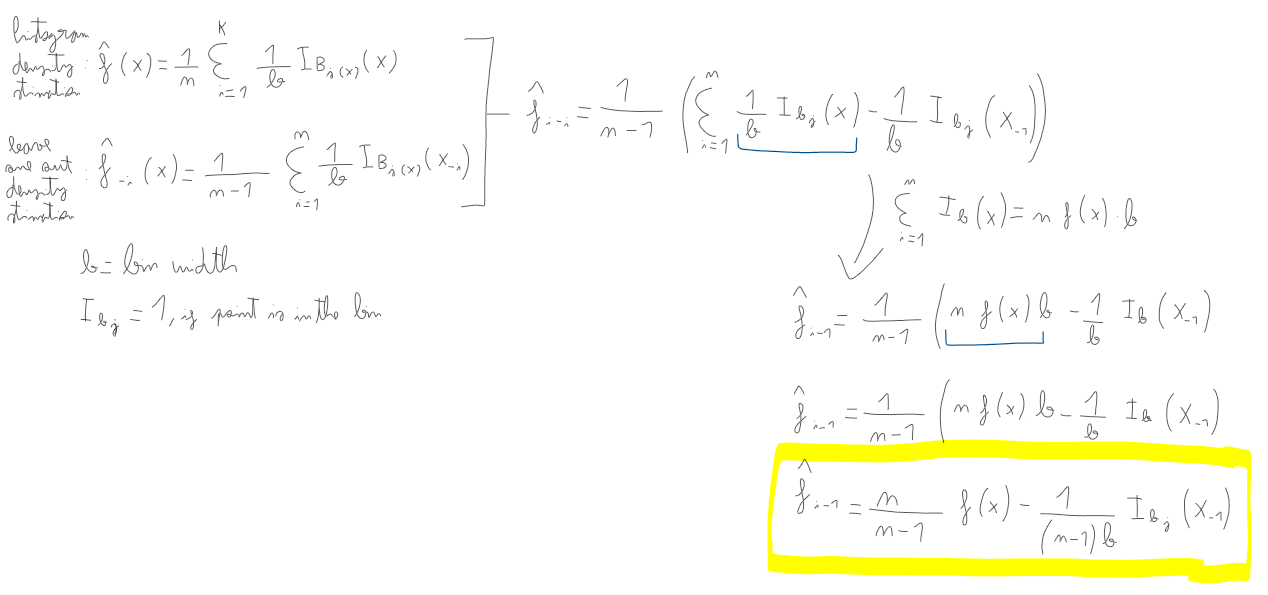
\includegraphics{Exercise_1.PNG}

\section{Exercise 2-3}\label{exercise-2-3}

\begin{Shaded}
\begin{Highlighting}[]
\CommentTok{\# Read and transform x to numeric}
\NormalTok{df }\OtherTok{=} \FunctionTok{read.table}\NormalTok{(}\StringTok{"cdrate.dat"}\NormalTok{, }\AttributeTok{col.names =} \FunctionTok{c}\NormalTok{(}\StringTok{"x"}\NormalTok{, }\StringTok{"y"}\NormalTok{))}
\NormalTok{x }\OtherTok{=}\NormalTok{ df[}\StringTok{"x"}\NormalTok{]}
\FunctionTok{class}\NormalTok{(x) }\OtherTok{=} \StringTok{"Numeric"}
\NormalTok{x }\OtherTok{=}\NormalTok{ x}\SpecialCharTok{$}\NormalTok{x}

\NormalTok{A }\OtherTok{\textless{}{-}} \FunctionTok{min}\NormalTok{(x)}\SpecialCharTok{{-}}\NormalTok{.}\DecValTok{05}\SpecialCharTok{*}\FunctionTok{diff}\NormalTok{(}\FunctionTok{range}\NormalTok{(x))}
\NormalTok{Z }\OtherTok{\textless{}{-}} \FunctionTok{max}\NormalTok{(x)}\SpecialCharTok{+}\NormalTok{.}\DecValTok{05}\SpecialCharTok{*}\FunctionTok{diff}\NormalTok{(}\FunctionTok{range}\NormalTok{(x))}
\NormalTok{nbr }\OtherTok{\textless{}{-}} \DecValTok{7}

\CommentTok{\# Define histogram and the function}
\NormalTok{hx }\OtherTok{\textless{}{-}} \FunctionTok{hist}\NormalTok{(x,}\AttributeTok{breaks=}\FunctionTok{seq}\NormalTok{(A,Z,}\AttributeTok{length=}\NormalTok{nbr}\SpecialCharTok{+}\DecValTok{1}\NormalTok{),}\AttributeTok{freq=}\NormalTok{F, }\AttributeTok{main =} \StringTok{"Original data"}\NormalTok{)}

\NormalTok{hx\_f }\OtherTok{\textless{}{-}} \FunctionTok{stepfun}\NormalTok{(hx}\SpecialCharTok{$}\NormalTok{breaks,}\FunctionTok{c}\NormalTok{(}\DecValTok{0}\NormalTok{,hx}\SpecialCharTok{$}\NormalTok{density,}\DecValTok{0}\NormalTok{))}
\NormalTok{binwidth }\OtherTok{\textless{}{-}}\NormalTok{ hx}\SpecialCharTok{$}\NormalTok{breaks[}\DecValTok{2}\NormalTok{]}\SpecialCharTok{{-}}\NormalTok{hx}\SpecialCharTok{$}\NormalTok{breaks[}\DecValTok{1}\NormalTok{]}
\FunctionTok{points}\NormalTok{(x,}\FunctionTok{hx\_f}\NormalTok{(x),}\AttributeTok{col=}\StringTok{"red"}\NormalTok{, }\AttributeTok{pch=}\DecValTok{1}\NormalTok{)}

\NormalTok{y\_loo\_hist }\OtherTok{\textless{}{-}}\NormalTok{ (}\FunctionTok{hx\_f}\NormalTok{(x)}\SpecialCharTok{{-}}\NormalTok{(}\DecValTok{1}\SpecialCharTok{/}\NormalTok{(}\FunctionTok{length}\NormalTok{(x)}\SpecialCharTok{*}\NormalTok{binwidth)))}\SpecialCharTok{*}\NormalTok{(}\FunctionTok{length}\NormalTok{(x)}\SpecialCharTok{/}\NormalTok{(}\FunctionTok{length}\NormalTok{(x)}\SpecialCharTok{{-}}\DecValTok{1}\NormalTok{))}
\FunctionTok{points}\NormalTok{(x,y\_loo\_hist,}\AttributeTok{col=}\StringTok{"black"}\NormalTok{, }\AttributeTok{pch=}\DecValTok{1}\NormalTok{)}

\FunctionTok{legend}\NormalTok{(}\StringTok{"topleft"}\NormalTok{, }\AttributeTok{legend =} \FunctionTok{c}\NormalTok{(}\StringTok{"f\_histogram"}\NormalTok{, }\StringTok{"l{-}o{-}o"}\NormalTok{), }\AttributeTok{col =} \FunctionTok{c}\NormalTok{(}\StringTok{"red"}\NormalTok{, }\StringTok{"black"}\NormalTok{), }\AttributeTok{pch =} \DecValTok{1}\NormalTok{, }\AttributeTok{bty =} \StringTok{"n"}\NormalTok{)}
\end{Highlighting}
\end{Shaded}

\includegraphics{Delivery1_files/figure-latex/unnamed-chunk-1-1.pdf}

\section{Exercise 4}\label{exercise-4}

The leave-one-out log-likelihood is calculated by the function
\(l_{C V}(b)=\sum_{i=1}^n \log \hat{f}_{hist,(-i)}\left(x_i\right)\).

\begin{Shaded}
\begin{Highlighting}[]
\NormalTok{l }\OtherTok{\textless{}{-}} \FunctionTok{sum}\NormalTok{(}\FunctionTok{log}\NormalTok{(y\_loo\_hist))}
\FunctionTok{print}\NormalTok{(}\StringTok{"The leave{-}one{-}out log{-}likelihood is:"}\NormalTok{)}
\end{Highlighting}
\end{Shaded}

\begin{verbatim}
## [1] "The leave-one-out log-likelihood is:"
\end{verbatim}

\begin{Shaded}
\begin{Highlighting}[]
\FunctionTok{print}\NormalTok{(l)}
\end{Highlighting}
\end{Shaded}

\begin{verbatim}
## [1] -16.58432
\end{verbatim}

\section{Exercise 5}\label{exercise-5}

For exercise 5, we determined the optimal number of histogram intervals
(nbr) by calculating the leave-one-out log-likelihood for different
values of nbr ranging from 1 to 15. We then selected the value that
maximized the log-likelihood as the optimal choice, and used this to
plot the final histogram.

\begin{Shaded}
\begin{Highlighting}[]
\NormalTok{nbr\_seq }\OtherTok{\textless{}{-}} \FunctionTok{seq}\NormalTok{(}\DecValTok{1}\NormalTok{, }\DecValTok{15}\NormalTok{)}
\NormalTok{looCV\_log\_lik }\OtherTok{\textless{}{-}} \FunctionTok{numeric}\NormalTok{(}\FunctionTok{length}\NormalTok{(nbr\_seq))  }\CommentTok{\# Pre{-}allocate for efficiency}

\CommentTok{\# Loop through each value of nbr}
\ControlFlowTok{for}\NormalTok{ (i }\ControlFlowTok{in} \FunctionTok{seq\_along}\NormalTok{(nbr\_seq)) \{}
\NormalTok{  nbr }\OtherTok{\textless{}{-}}\NormalTok{ nbr\_seq[i]}
  
  \CommentTok{\# Compute the histogram}
\NormalTok{  hx }\OtherTok{\textless{}{-}} \FunctionTok{hist}\NormalTok{(x, }\AttributeTok{breaks =} \FunctionTok{seq}\NormalTok{(A, Z, }\AttributeTok{length =}\NormalTok{ nbr }\SpecialCharTok{+} \DecValTok{1}\NormalTok{), }\AttributeTok{plot =} \ConstantTok{FALSE}\NormalTok{)}
\NormalTok{  binwidth }\OtherTok{\textless{}{-}}\NormalTok{ hx}\SpecialCharTok{$}\NormalTok{breaks[}\DecValTok{2}\NormalTok{] }\SpecialCharTok{{-}}\NormalTok{ hx}\SpecialCharTok{$}\NormalTok{breaks[}\DecValTok{1}\NormalTok{]  }\CommentTok{\# Calculate bin width}
  
  \CommentTok{\# Convert histogram into a step function and evaluate the leave{-}one{-}out estimate}
\NormalTok{  hx\_f }\OtherTok{\textless{}{-}} \FunctionTok{stepfun}\NormalTok{(hx}\SpecialCharTok{$}\NormalTok{breaks, }\FunctionTok{c}\NormalTok{(}\DecValTok{0}\NormalTok{, hx}\SpecialCharTok{$}\NormalTok{density, }\DecValTok{0}\NormalTok{))}
\NormalTok{  y\_loo\_hist }\OtherTok{\textless{}{-}}\NormalTok{ (}\FunctionTok{hx\_f}\NormalTok{(x) }\SpecialCharTok{{-}}\NormalTok{ (}\DecValTok{1} \SpecialCharTok{/}\NormalTok{ (}\FunctionTok{length}\NormalTok{(x) }\SpecialCharTok{*}\NormalTok{ binwidth))) }\SpecialCharTok{*}\NormalTok{ (}\FunctionTok{length}\NormalTok{(x) }\SpecialCharTok{/}\NormalTok{ (}\FunctionTok{length}\NormalTok{(x) }\SpecialCharTok{{-}} \DecValTok{1}\NormalTok{))}
  
  \CommentTok{\# Calculate the log{-}likelihood and handle zero values}
  \ControlFlowTok{if}\NormalTok{ (}\FunctionTok{any}\NormalTok{(y\_loo\_hist }\SpecialCharTok{\textless{}=} \DecValTok{0}\NormalTok{)) \{}
\NormalTok{    looCV\_log\_lik[i] }\OtherTok{\textless{}{-}} \SpecialCharTok{{-}}\ConstantTok{Inf}
\NormalTok{  \} }\ControlFlowTok{else}\NormalTok{ \{}
\NormalTok{    looCV\_log\_lik[i] }\OtherTok{\textless{}{-}} \FunctionTok{sum}\NormalTok{(}\FunctionTok{log}\NormalTok{(y\_loo\_hist))}
\NormalTok{  \}}
\NormalTok{\}}

\CommentTok{\# Identify the optimal number of bins}
\NormalTok{optimal\_nbr }\OtherTok{\textless{}{-}}\NormalTok{ nbr\_seq[}\FunctionTok{which.max}\NormalTok{(looCV\_log\_lik)]}
\NormalTok{optimal\_log\_lik }\OtherTok{\textless{}{-}} \FunctionTok{max}\NormalTok{(looCV\_log\_lik)}

\CommentTok{\# Plot the leave{-}one{-}out log{-}likelihood with a marker for the optimal bin count}
\FunctionTok{plot}\NormalTok{(nbr\_seq, looCV\_log\_lik, }\AttributeTok{type =} \StringTok{"b"}\NormalTok{, }\AttributeTok{xlab =} \StringTok{\textquotesingle{}Number of Bins\textquotesingle{}}\NormalTok{, }\AttributeTok{ylab =} \StringTok{\textquotesingle{}Log Likelihood (Leave{-}One{-}Out)\textquotesingle{}}\NormalTok{,}
     \AttributeTok{main =} \StringTok{"Leave{-}One{-}Out Log Likelihood vs Number of Bins"}\NormalTok{)}

\CommentTok{\# Highlight the optimal number of bins on the plot}
\FunctionTok{points}\NormalTok{(optimal\_nbr, optimal\_log\_lik, }\AttributeTok{col =} \StringTok{"red"}\NormalTok{, }\AttributeTok{pch =} \DecValTok{19}\NormalTok{, }\AttributeTok{cex =} \FloatTok{1.5}\NormalTok{)  }\CommentTok{\# Red dot for maximum}
\FunctionTok{text}\NormalTok{(optimal\_nbr, optimal\_log\_lik, }\AttributeTok{labels =} \FunctionTok{paste}\NormalTok{(}\StringTok{"Best nbr ="}\NormalTok{, optimal\_nbr), }\AttributeTok{pos =} \DecValTok{3}\NormalTok{, }\AttributeTok{col =} \StringTok{"red"}\NormalTok{)}
\end{Highlighting}
\end{Shaded}

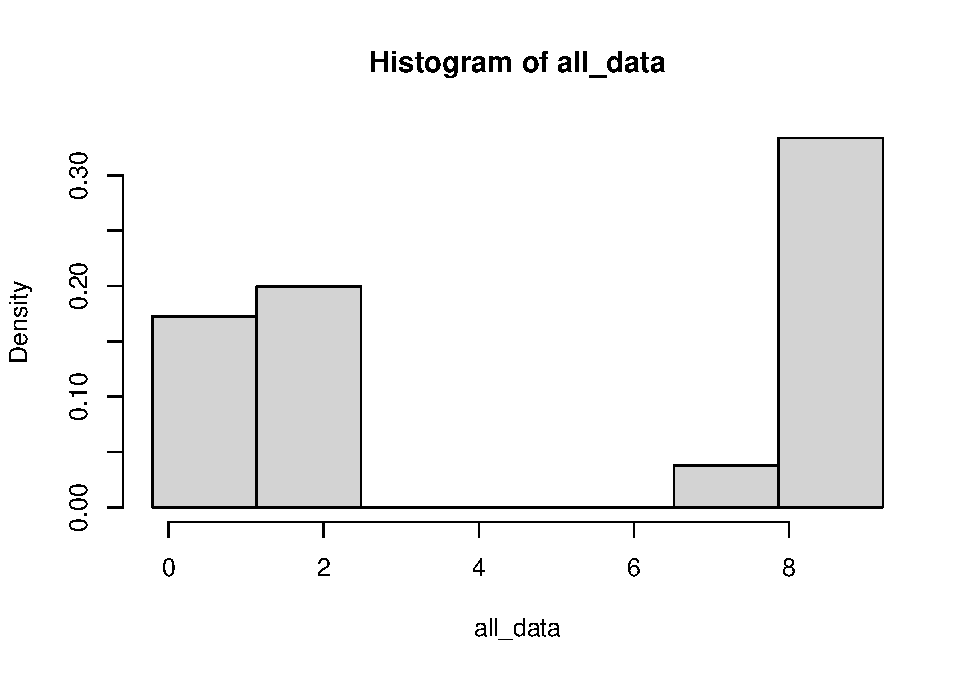
\includegraphics{Delivery1_files/figure-latex/unnamed-chunk-3-1.pdf}

\section{Exercise 6}\label{exercise-6}

Here we followed a similar approach to exercise 5, but focused on
finding the optimal bin width (b). We evaluated the leave-one-out
log-likelihood for a range of possible bin widths and chose the one that
maximized the log-likelihood. The histogram was then plotted using this
optimal bin width.

\begin{Shaded}
\begin{Highlighting}[]
\NormalTok{b\_seq }\OtherTok{\textless{}{-}} \FunctionTok{seq}\NormalTok{((Z }\SpecialCharTok{{-}}\NormalTok{ A) }\SpecialCharTok{/} \DecValTok{15}\NormalTok{, (Z }\SpecialCharTok{{-}}\NormalTok{ A), }\AttributeTok{length =} \DecValTok{30}\NormalTok{)}
\NormalTok{looCV\_log\_lik }\OtherTok{\textless{}{-}} \FunctionTok{numeric}\NormalTok{(}\FunctionTok{length}\NormalTok{(b\_seq))  }\CommentTok{\# Pre{-}allocate for efficiency}

\CommentTok{\# Loop through each bin width b}
\ControlFlowTok{for}\NormalTok{ (i }\ControlFlowTok{in} \FunctionTok{seq\_along}\NormalTok{(b\_seq)) \{}
\NormalTok{  b }\OtherTok{\textless{}{-}}\NormalTok{ b\_seq[i]}
  
  \CommentTok{\# Compute the histogram with the specified bin width b}
\NormalTok{  hx }\OtherTok{\textless{}{-}} \FunctionTok{hist}\NormalTok{(x, }\AttributeTok{breaks =} \FunctionTok{seq}\NormalTok{(A, Z }\SpecialCharTok{+}\NormalTok{ b, }\AttributeTok{by =}\NormalTok{ b), }\AttributeTok{plot =} \ConstantTok{FALSE}\NormalTok{)}
\NormalTok{  binwidth }\OtherTok{\textless{}{-}} \FunctionTok{diff}\NormalTok{(hx}\SpecialCharTok{$}\NormalTok{breaks)[}\DecValTok{1}\NormalTok{]  }\CommentTok{\# Confirming the bin width}
  
  \CommentTok{\# Convert histogram into a step function and evaluate at data points}
\NormalTok{  hx\_f }\OtherTok{\textless{}{-}} \FunctionTok{stepfun}\NormalTok{(hx}\SpecialCharTok{$}\NormalTok{breaks, }\FunctionTok{c}\NormalTok{(}\DecValTok{0}\NormalTok{, hx}\SpecialCharTok{$}\NormalTok{density, }\DecValTok{0}\NormalTok{))}
\NormalTok{  y\_hist }\OtherTok{\textless{}{-}} \FunctionTok{hx\_f}\NormalTok{(x)}
  
  \CommentTok{\# Compute the leave{-}one{-}out histogram estimate}
\NormalTok{  y\_loo\_hist }\OtherTok{\textless{}{-}}\NormalTok{ (y\_hist }\SpecialCharTok{{-}}\NormalTok{ (}\DecValTok{1} \SpecialCharTok{/}\NormalTok{ (}\FunctionTok{length}\NormalTok{(x) }\SpecialCharTok{*}\NormalTok{ binwidth))) }\SpecialCharTok{*}\NormalTok{ (}\FunctionTok{length}\NormalTok{(x) }\SpecialCharTok{/}\NormalTok{ (}\FunctionTok{length}\NormalTok{(x) }\SpecialCharTok{{-}} \DecValTok{1}\NormalTok{))}
  
  \CommentTok{\# Calculate log{-}likelihood, handling cases with zero or negative values}
  \ControlFlowTok{if}\NormalTok{ (}\FunctionTok{any}\NormalTok{(y\_loo\_hist }\SpecialCharTok{\textless{}=} \DecValTok{0}\NormalTok{)) \{}
\NormalTok{    looCV\_log\_lik[i] }\OtherTok{\textless{}{-}} \SpecialCharTok{{-}}\ConstantTok{Inf}
\NormalTok{  \} }\ControlFlowTok{else}\NormalTok{ \{}
\NormalTok{    looCV\_log\_lik[i] }\OtherTok{\textless{}{-}} \FunctionTok{sum}\NormalTok{(}\FunctionTok{log}\NormalTok{(y\_loo\_hist))}
\NormalTok{  \}}
\NormalTok{\}}

\CommentTok{\# Identify the optimal bin width}
\NormalTok{optimal\_b }\OtherTok{\textless{}{-}}\NormalTok{ b\_seq[}\FunctionTok{which.max}\NormalTok{(looCV\_log\_lik)]}
\NormalTok{optimal\_log\_lik }\OtherTok{\textless{}{-}} \FunctionTok{max}\NormalTok{(looCV\_log\_lik)}

\CommentTok{\# Plot the leave{-}one{-}out log{-}likelihoods for different bin widths}
\FunctionTok{plot}\NormalTok{(b\_seq, looCV\_log\_lik, }\AttributeTok{type =} \StringTok{"b"}\NormalTok{, }\AttributeTok{xlab =} \StringTok{\textquotesingle{}Bin Width (b)\textquotesingle{}}\NormalTok{, }\AttributeTok{ylab =} \StringTok{\textquotesingle{}Log Likelihood (Leave{-}One{-}Out)\textquotesingle{}}\NormalTok{,}
     \AttributeTok{main =} \StringTok{"Leave{-}One{-}Out Log Likelihood vs Bin Width"}\NormalTok{, }\AttributeTok{col =} \StringTok{"blue"}\NormalTok{, }\AttributeTok{pch =} \DecValTok{19}\NormalTok{)}

\CommentTok{\# Highlight the optimal bin width on the plot}
\FunctionTok{points}\NormalTok{(optimal\_b, optimal\_log\_lik, }\AttributeTok{col =} \StringTok{"red"}\NormalTok{, }\AttributeTok{pch =} \DecValTok{19}\NormalTok{, }\AttributeTok{cex =} \FloatTok{1.5}\NormalTok{)}
\FunctionTok{text}\NormalTok{(optimal\_b, optimal\_log\_lik, }\AttributeTok{labels =} \FunctionTok{paste}\NormalTok{(}\StringTok{"Best b ="}\NormalTok{, }\FunctionTok{round}\NormalTok{(optimal\_b, }\DecValTok{3}\NormalTok{)), }\AttributeTok{pos =} \DecValTok{3}\NormalTok{, }\AttributeTok{col =} \StringTok{"red"}\NormalTok{)}
\end{Highlighting}
\end{Shaded}

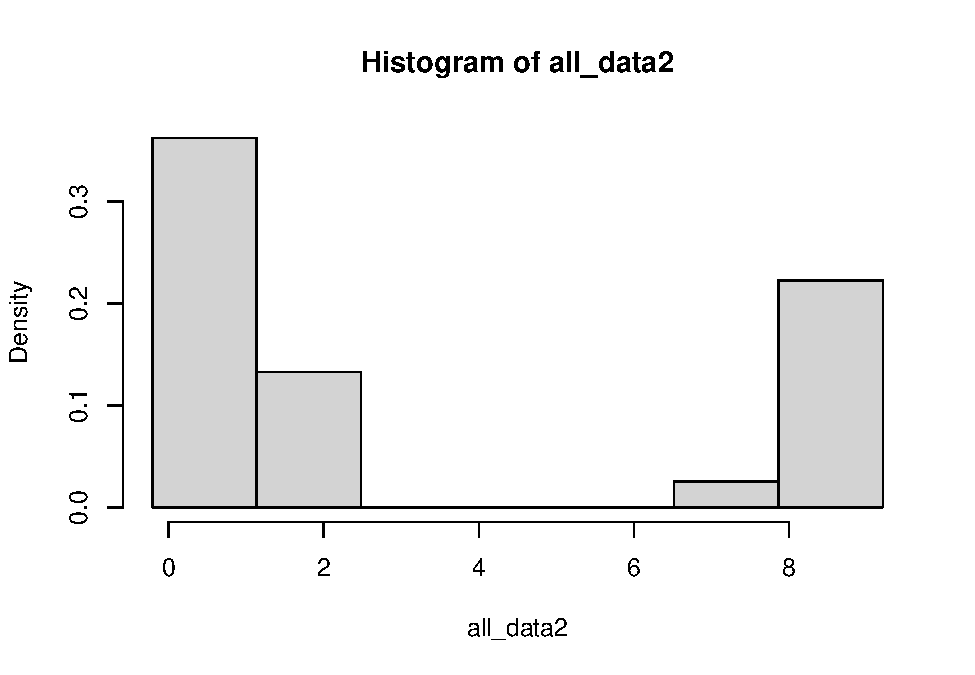
\includegraphics{Delivery1_files/figure-latex/unnamed-chunk-4-1.pdf}

\begin{Shaded}
\begin{Highlighting}[]
\CommentTok{\# Plot the histogram using the optimal bin width}
\FunctionTok{hist}\NormalTok{(x, }\AttributeTok{breaks =} \FunctionTok{seq}\NormalTok{(A, Z }\SpecialCharTok{+}\NormalTok{ optimal\_b, }\AttributeTok{by =}\NormalTok{ optimal\_b), }\AttributeTok{freq =} \ConstantTok{FALSE}\NormalTok{, }
     \AttributeTok{main =} \FunctionTok{paste}\NormalTok{(}\StringTok{"Optimal Histogram with Bin Width ="}\NormalTok{, }\FunctionTok{round}\NormalTok{(optimal\_b, }\DecValTok{3}\NormalTok{)), }
     \AttributeTok{xlab =} \StringTok{"Data"}\NormalTok{, }\AttributeTok{ylab =} \StringTok{"Density"}\NormalTok{, }\AttributeTok{col =} \StringTok{"lightgray"}\NormalTok{, }\AttributeTok{border =} \StringTok{"darkgray"}\NormalTok{)}
\end{Highlighting}
\end{Shaded}

\includegraphics{Delivery1_files/figure-latex/unnamed-chunk-4-2.pdf}

\section{Exercise 7}\label{exercise-7}

Generate \(n=100\) data from \[
f(x) = (3/4)N(x; m = 0, s = 1) +(1/4) N(x; m = 3/2, s = 1/3)\]

\begin{Shaded}
\begin{Highlighting}[]
\FunctionTok{par}\NormalTok{(}\AttributeTok{mfrow=}\FunctionTok{c}\NormalTok{(}\DecValTok{1}\NormalTok{,}\DecValTok{1}\NormalTok{))}

\NormalTok{sim.mixt }\OtherTok{\textless{}{-}} \ControlFlowTok{function}\NormalTok{(}\AttributeTok{n=}\DecValTok{1}\NormalTok{,}\AttributeTok{k=}\DecValTok{1}\NormalTok{, }
         \AttributeTok{mu=}\FunctionTok{seq}\NormalTok{(}\SpecialCharTok{{-}}\DecValTok{2}\SpecialCharTok{*}\NormalTok{(k}\DecValTok{{-}1}\NormalTok{),}\DecValTok{2}\SpecialCharTok{*}\NormalTok{(k}\DecValTok{{-}1}\NormalTok{),}\AttributeTok{length=}\NormalTok{k), }
         \AttributeTok{sigma=}\FunctionTok{seq}\NormalTok{(}\DecValTok{1}\NormalTok{,}\DecValTok{1}\NormalTok{,}\AttributeTok{length=}\NormalTok{k), }
         \AttributeTok{alpha=}\FunctionTok{seq}\NormalTok{(}\DecValTok{1}\SpecialCharTok{/}\NormalTok{k,}\DecValTok{1}\SpecialCharTok{/}\NormalTok{k,}\AttributeTok{length=}\NormalTok{k), }\AttributeTok{graphic=}\ConstantTok{FALSE}\NormalTok{,...)}
\NormalTok{\{}
\NormalTok{   csa}\OtherTok{\textless{}{-}}\FunctionTok{cumsum}\NormalTok{(alpha)}
\NormalTok{   x}\OtherTok{\textless{}{-}}\FunctionTok{runif}\NormalTok{(n)}
      
   \ControlFlowTok{for}\NormalTok{ (i }\ControlFlowTok{in} \DecValTok{1}\SpecialCharTok{:}\NormalTok{n)\{}
\NormalTok{      comp}\OtherTok{\textless{}{-}}\FunctionTok{sum}\NormalTok{(csa}\SpecialCharTok{\textless{}=}\NormalTok{x[i])}\SpecialCharTok{+}\DecValTok{1}
\NormalTok{      x[i]}\OtherTok{\textless{}{-}}\FunctionTok{rnorm}\NormalTok{(}\DecValTok{1}\NormalTok{,mu[comp],sigma[comp])}
\NormalTok{   \}}
   \ControlFlowTok{if}\NormalTok{(graphic) \{}
\NormalTok{      out}\OtherTok{\textless{}{-}}\FunctionTok{graph.mixt}\NormalTok{(k, mu, sigma, alpha, }\AttributeTok{gr=}\ConstantTok{FALSE}\NormalTok{)}
      \FunctionTok{hist}\NormalTok{(x,}\AttributeTok{freq =} \ConstantTok{FALSE}\NormalTok{,}
           \AttributeTok{ylim=}\FunctionTok{c}\NormalTok{(}\DecValTok{0}\NormalTok{,}\FunctionTok{max}\NormalTok{(}\FunctionTok{c}\NormalTok{(}\FunctionTok{max}\NormalTok{(out}\SpecialCharTok{$}\NormalTok{fx),}\FunctionTok{max}\NormalTok{(}\FunctionTok{hist}\NormalTok{(x,}\AttributeTok{plot=}\ConstantTok{FALSE}\NormalTok{)}\SpecialCharTok{$}\NormalTok{density)))))}
      \FunctionTok{lines}\NormalTok{(out}\SpecialCharTok{$}\NormalTok{x,out}\SpecialCharTok{$}\NormalTok{fx,}\AttributeTok{lty=}\DecValTok{1}\NormalTok{,}\AttributeTok{lwd=}\DecValTok{2}\NormalTok{)}
\NormalTok{   \}   }
   \FunctionTok{return}\NormalTok{(x)}
\NormalTok{\}}

\NormalTok{graph.mixt}\OtherTok{\textless{}{-}}\ControlFlowTok{function}\NormalTok{(}\AttributeTok{k=}\DecValTok{1}\NormalTok{, }\AttributeTok{mu=}\FunctionTok{seq}\NormalTok{(}\SpecialCharTok{{-}}\DecValTok{2}\SpecialCharTok{*}\NormalTok{(k}\DecValTok{{-}1}\NormalTok{),}\DecValTok{2}\SpecialCharTok{*}\NormalTok{(k}\DecValTok{{-}1}\NormalTok{),}\AttributeTok{length=}\NormalTok{k), }\AttributeTok{sigma=}\FunctionTok{seq}\NormalTok{(}\DecValTok{1}\NormalTok{,}\DecValTok{1}\NormalTok{,}\AttributeTok{length=}\NormalTok{k), }\AttributeTok{alpha=}\FunctionTok{seq}\NormalTok{(}\DecValTok{1}\SpecialCharTok{/}\NormalTok{k,}\DecValTok{1}\SpecialCharTok{/}\NormalTok{k,}\AttributeTok{length=}\NormalTok{k), }\AttributeTok{graphic=}\ConstantTok{TRUE}\NormalTok{,...)}
\NormalTok{\{}
\NormalTok{   L}\OtherTok{\textless{}{-}}\FunctionTok{min}\NormalTok{(mu}\DecValTok{{-}3}\SpecialCharTok{*}\NormalTok{sigma)}
\NormalTok{   U}\OtherTok{\textless{}{-}}\FunctionTok{max}\NormalTok{(mu}\SpecialCharTok{+}\DecValTok{3}\SpecialCharTok{*}\NormalTok{sigma)}
         
\NormalTok{   x}\OtherTok{\textless{}{-}} \FunctionTok{seq}\NormalTok{(}\AttributeTok{from=}\NormalTok{L,}\AttributeTok{to=}\NormalTok{U,}\AttributeTok{length=}\DecValTok{200}\NormalTok{)}
\NormalTok{   fx}\OtherTok{\textless{}{-}} \DecValTok{0}\SpecialCharTok{*}\NormalTok{x}
\NormalTok{   Salpha}\OtherTok{\textless{}{-}}\FunctionTok{sum}\NormalTok{(alpha)}
   \ControlFlowTok{for}\NormalTok{(i }\ControlFlowTok{in} \DecValTok{1}\SpecialCharTok{:}\NormalTok{k)\{}
\NormalTok{    p}\OtherTok{\textless{}{-}}\NormalTok{alpha[i]}\SpecialCharTok{/}\NormalTok{Salpha}
\CommentTok{\#       fx \textless{}{-} fx + p*exp({-}.5*((x{-}mu[i])/sigma[i])\^{}2)/(sqrt(2*pi)*sigma[i])}
\NormalTok{    fx }\OtherTok{\textless{}{-}}\NormalTok{ fx }\SpecialCharTok{+}\NormalTok{ p}\SpecialCharTok{*}\FunctionTok{dnorm}\NormalTok{(x,mu[i],sigma[i])}
\NormalTok{   \}}
   \ControlFlowTok{if}\NormalTok{ (graphic)\{}
      \FunctionTok{plot}\NormalTok{(x,fx,}\AttributeTok{type=}\StringTok{"l"}\NormalTok{,...)}
\NormalTok{   \}}
   \FunctionTok{return}\NormalTok{(}\FunctionTok{list}\NormalTok{(}\AttributeTok{L =}\NormalTok{ L, }\AttributeTok{U =}\NormalTok{ U, }\AttributeTok{x =}\NormalTok{ x, }\AttributeTok{fx =}\NormalTok{ fx))}
\NormalTok{\}}

\FunctionTok{set.seed}\NormalTok{(}\DecValTok{123}\NormalTok{)}
\NormalTok{n }\OtherTok{\textless{}{-}} \DecValTok{100}
\NormalTok{x }\OtherTok{\textless{}{-}} \FunctionTok{sim.mixt}\NormalTok{(}\AttributeTok{n =}\NormalTok{ n, }\AttributeTok{k =} \DecValTok{2}\NormalTok{, }\AttributeTok{mu =} \FunctionTok{c}\NormalTok{(}\DecValTok{0}\NormalTok{, }\FloatTok{1.5}\NormalTok{), }\AttributeTok{sigma =} \FunctionTok{c}\NormalTok{(}\DecValTok{1}\NormalTok{, }\DecValTok{1}\SpecialCharTok{/}\DecValTok{3}\NormalTok{), }\AttributeTok{alpha =} \FunctionTok{c}\NormalTok{(}\DecValTok{3}\SpecialCharTok{/}\DecValTok{4}\NormalTok{, }\DecValTok{1}\SpecialCharTok{/}\DecValTok{4}\NormalTok{))}

\NormalTok{A }\OtherTok{\textless{}{-}} \FunctionTok{min}\NormalTok{(x) }\SpecialCharTok{{-}} \FloatTok{0.05} \SpecialCharTok{*} \FunctionTok{diff}\NormalTok{(}\FunctionTok{range}\NormalTok{(x))}
\NormalTok{Z }\OtherTok{\textless{}{-}} \FunctionTok{max}\NormalTok{(x) }\SpecialCharTok{+} \FloatTok{0.05} \SpecialCharTok{*} \FunctionTok{diff}\NormalTok{(}\FunctionTok{range}\NormalTok{(x))}

\NormalTok{sigma.mixt }\OtherTok{\textless{}{-}} \FloatTok{1.095287}
\NormalTok{scott\_b }\OtherTok{\textless{}{-}} \FloatTok{3.49} \SpecialCharTok{*}\NormalTok{ sigma.mixt }\SpecialCharTok{*} \FunctionTok{length}\NormalTok{(x)}\SpecialCharTok{\^{}}\NormalTok{(}\SpecialCharTok{{-}}\DecValTok{1}\SpecialCharTok{/}\DecValTok{3}\NormalTok{)}
\end{Highlighting}
\end{Shaded}

We use the Scott's formula to find the value of b = \texttt{r}scott\_b`
(this was done in the density estimation script used in class). The
following is the histogram result:

\begin{Shaded}
\begin{Highlighting}[]
\NormalTok{hx }\OtherTok{\textless{}{-}} \FunctionTok{hist}\NormalTok{(x,}\AttributeTok{breaks=}\FunctionTok{seq}\NormalTok{(A,Z}\SpecialCharTok{+}\NormalTok{b,}\AttributeTok{by=}\NormalTok{scott\_b), }\AttributeTok{plot=}\NormalTok{F)}
\FunctionTok{plot}\NormalTok{(hx,}\AttributeTok{freq =} \ConstantTok{FALSE}\NormalTok{)}
\end{Highlighting}
\end{Shaded}

\includegraphics{Delivery1_files/figure-latex/unnamed-chunk-6-1.pdf}

Now taking the b value maximizing the leave-one-out log-likelihood
function. The sequence of proposed b-values to select from is varied
from 0.05 to 1.75 in steps of 0.01.

\begin{Shaded}
\begin{Highlighting}[]
\NormalTok{b\_seq }\OtherTok{\textless{}{-}} \FunctionTok{seq}\NormalTok{((Z }\SpecialCharTok{{-}}\NormalTok{ A) }\SpecialCharTok{/} \DecValTok{15}\NormalTok{, (Z }\SpecialCharTok{{-}}\NormalTok{ A), }\AttributeTok{length =} \DecValTok{30}\NormalTok{)}
\NormalTok{looCV\_log\_lik }\OtherTok{\textless{}{-}} \FunctionTok{numeric}\NormalTok{(}\FunctionTok{length}\NormalTok{(b\_seq))}

\ControlFlowTok{for}\NormalTok{ (i }\ControlFlowTok{in} \FunctionTok{seq\_along}\NormalTok{(b\_seq)) \{}
\NormalTok{  b }\OtherTok{\textless{}{-}}\NormalTok{ b\_seq[i]}
  
  \CommentTok{\# Compute the histogram with the specified bin width b}
\NormalTok{  hx }\OtherTok{\textless{}{-}} \FunctionTok{hist}\NormalTok{(x, }\AttributeTok{breaks =} \FunctionTok{seq}\NormalTok{(A, Z }\SpecialCharTok{+}\NormalTok{ b, }\AttributeTok{by =}\NormalTok{ b), }\AttributeTok{plot =} \ConstantTok{FALSE}\NormalTok{)}
\NormalTok{  binwidth }\OtherTok{\textless{}{-}} \FunctionTok{diff}\NormalTok{(hx}\SpecialCharTok{$}\NormalTok{breaks)[}\DecValTok{1}\NormalTok{]  }\CommentTok{\# Confirm the bin width}
  
  \CommentTok{\# Convert histogram into a step function and evaluate at data points}
\NormalTok{  hx\_f }\OtherTok{\textless{}{-}} \FunctionTok{stepfun}\NormalTok{(hx}\SpecialCharTok{$}\NormalTok{breaks, }\FunctionTok{c}\NormalTok{(}\DecValTok{0}\NormalTok{, hx}\SpecialCharTok{$}\NormalTok{density, }\DecValTok{0}\NormalTok{))}
\NormalTok{  y\_hist }\OtherTok{\textless{}{-}} \FunctionTok{hx\_f}\NormalTok{(x)}
  
  \CommentTok{\# Compute the leave{-}one{-}out histogram estimate}
\NormalTok{  y\_loo\_hist }\OtherTok{\textless{}{-}}\NormalTok{ (y\_hist }\SpecialCharTok{{-}}\NormalTok{ (}\DecValTok{1} \SpecialCharTok{/}\NormalTok{ (n }\SpecialCharTok{*}\NormalTok{ binwidth))) }\SpecialCharTok{*}\NormalTok{ (n }\SpecialCharTok{/}\NormalTok{ (n }\SpecialCharTok{{-}} \DecValTok{1}\NormalTok{))}
  
  \CommentTok{\# Calculate log{-}likelihood, handling cases with zero or negative values}
  \ControlFlowTok{if}\NormalTok{ (}\FunctionTok{any}\NormalTok{(y\_loo\_hist }\SpecialCharTok{\textless{}=} \DecValTok{0}\NormalTok{)) \{}
\NormalTok{    looCV\_log\_lik[i] }\OtherTok{\textless{}{-}} \SpecialCharTok{{-}}\ConstantTok{Inf}
\NormalTok{  \} }\ControlFlowTok{else}\NormalTok{ \{}
\NormalTok{    looCV\_log\_lik[i] }\OtherTok{\textless{}{-}} \FunctionTok{sum}\NormalTok{(}\FunctionTok{log}\NormalTok{(y\_loo\_hist))}
\NormalTok{  \}}
\NormalTok{\}}

\FunctionTok{par}\NormalTok{(}\AttributeTok{mfrow=}\FunctionTok{c}\NormalTok{(}\DecValTok{1}\NormalTok{,}\DecValTok{1}\NormalTok{))}

\NormalTok{optimal\_b }\OtherTok{\textless{}{-}}\NormalTok{ b\_seq[}\FunctionTok{which.max}\NormalTok{(looCV\_log\_lik)]}
\NormalTok{optimal\_log\_lik }\OtherTok{\textless{}{-}} \FunctionTok{max}\NormalTok{(looCV\_log\_lik)}

\FunctionTok{plot}\NormalTok{(b\_seq, looCV\_log\_lik, }\AttributeTok{type =} \StringTok{"b"}\NormalTok{, }\AttributeTok{xlab =} \StringTok{\textquotesingle{}Bin Width (b)\textquotesingle{}}\NormalTok{, }\AttributeTok{ylab =} \StringTok{\textquotesingle{}Log Likelihood (Leave{-}One{-}Out)\textquotesingle{}}\NormalTok{,}
     \AttributeTok{main =} \StringTok{"Leave{-}One{-}Out Log Likelihood vs Bin Width"}\NormalTok{, }\AttributeTok{col =} \StringTok{"blue"}\NormalTok{, }\AttributeTok{pch =} \DecValTok{19}\NormalTok{)}

\FunctionTok{points}\NormalTok{(optimal\_b, optimal\_log\_lik, }\AttributeTok{col =} \StringTok{"red"}\NormalTok{, }\AttributeTok{pch =} \DecValTok{19}\NormalTok{, }\AttributeTok{cex =} \FloatTok{1.5}\NormalTok{)}
\FunctionTok{text}\NormalTok{(optimal\_b, optimal\_log\_lik, }\AttributeTok{labels =} \FunctionTok{paste}\NormalTok{(}\StringTok{"Best b ="}\NormalTok{, }\FunctionTok{round}\NormalTok{(optimal\_b, }\DecValTok{3}\NormalTok{)), }\AttributeTok{pos =} \DecValTok{3}\NormalTok{, }\AttributeTok{col =} \StringTok{"red"}\NormalTok{)}
\FunctionTok{abline}\NormalTok{(}\AttributeTok{v =}\NormalTok{ scott\_b, }\AttributeTok{col =} \StringTok{"green"}\NormalTok{, }\AttributeTok{lwd =} \DecValTok{2}\NormalTok{, }\AttributeTok{lty =} \DecValTok{2}\NormalTok{)}
\FunctionTok{legend}\NormalTok{(}\StringTok{"topright"}\NormalTok{, }\AttributeTok{legend =} \FunctionTok{c}\NormalTok{(}\StringTok{"Optimal b (looCV)"}\NormalTok{, }\StringTok{"Scott\textquotesingle{}s b"}\NormalTok{), }\AttributeTok{col =} \FunctionTok{c}\NormalTok{(}\StringTok{"red"}\NormalTok{, }\StringTok{"green"}\NormalTok{), }\AttributeTok{pch =} \FunctionTok{c}\NormalTok{(}\DecValTok{19}\NormalTok{, }\ConstantTok{NA}\NormalTok{), }\AttributeTok{lty =} \FunctionTok{c}\NormalTok{(}\ConstantTok{NA}\NormalTok{, }\DecValTok{2}\NormalTok{))}
\end{Highlighting}
\end{Shaded}

\includegraphics{Delivery1_files/figure-latex/unnamed-chunk-7-1.pdf}

\begin{Shaded}
\begin{Highlighting}[]
\FunctionTok{hist}\NormalTok{(x, }\AttributeTok{breaks =} \FunctionTok{seq}\NormalTok{(A, Z }\SpecialCharTok{+}\NormalTok{ optimal\_b, }\AttributeTok{by =}\NormalTok{ optimal\_b), }\AttributeTok{freq =} \ConstantTok{FALSE}\NormalTok{, }
     \AttributeTok{main =} \FunctionTok{paste}\NormalTok{(}\StringTok{"Optimal Histogram with Bin Width ="}\NormalTok{, }\FunctionTok{round}\NormalTok{(optimal\_b, }\DecValTok{3}\NormalTok{)), }
     \AttributeTok{xlab =} \StringTok{"Data"}\NormalTok{, }\AttributeTok{ylab =} \StringTok{"Density"}\NormalTok{, }\AttributeTok{col =} \StringTok{"lightgray"}\NormalTok{, }\AttributeTok{border =} \StringTok{"darkgray"}\NormalTok{)}

\CommentTok{\# Overlay the mixture density from graph.mixt}
\NormalTok{mixture\_density }\OtherTok{\textless{}{-}} \FunctionTok{graph.mixt}\NormalTok{(}\AttributeTok{k =} \DecValTok{2}\NormalTok{, }\AttributeTok{mu =} \FunctionTok{c}\NormalTok{(}\DecValTok{0}\NormalTok{, }\FloatTok{1.5}\NormalTok{), }\AttributeTok{sigma =} \FunctionTok{c}\NormalTok{(}\DecValTok{1}\NormalTok{, }\DecValTok{1}\SpecialCharTok{/}\DecValTok{3}\NormalTok{), }\AttributeTok{alpha =} \FunctionTok{c}\NormalTok{(}\DecValTok{3}\SpecialCharTok{/}\DecValTok{4}\NormalTok{, }\DecValTok{1}\SpecialCharTok{/}\DecValTok{4}\NormalTok{), }\AttributeTok{graphic =} \ConstantTok{FALSE}\NormalTok{)}
\FunctionTok{lines}\NormalTok{(mixture\_density}\SpecialCharTok{$}\NormalTok{x, mixture\_density}\SpecialCharTok{$}\NormalTok{fx, }\AttributeTok{col =} \StringTok{"blue"}\NormalTok{, }\AttributeTok{lwd =} \DecValTok{2}\NormalTok{)}

\CommentTok{\# Annotate Scott\textquotesingle{}s bin width on the histogram}
\FunctionTok{abline}\NormalTok{(}\AttributeTok{v =}\NormalTok{ scott\_b, }\AttributeTok{col =} \StringTok{"green"}\NormalTok{, }\AttributeTok{lwd =} \DecValTok{2}\NormalTok{, }\AttributeTok{lty =} \DecValTok{2}\NormalTok{)}
\FunctionTok{text}\NormalTok{(scott\_b, }\FunctionTok{max}\NormalTok{(}\FunctionTok{hist}\NormalTok{(x, }\AttributeTok{breaks =} \FunctionTok{seq}\NormalTok{(A, Z }\SpecialCharTok{+}\NormalTok{ optimal\_b, }\AttributeTok{by =}\NormalTok{ optimal\_b), }\AttributeTok{plot =} \ConstantTok{FALSE}\NormalTok{)}\SpecialCharTok{$}\NormalTok{density) }\SpecialCharTok{*} \FloatTok{0.8}\NormalTok{,}
     \AttributeTok{labels =} \FunctionTok{paste}\NormalTok{(}\StringTok{"Scott\textquotesingle{}s b ="}\NormalTok{, }\FunctionTok{round}\NormalTok{(scott\_b, }\DecValTok{3}\NormalTok{)), }\AttributeTok{col =} \StringTok{"green"}\NormalTok{, }\AttributeTok{pos =} \DecValTok{4}\NormalTok{)}
\end{Highlighting}
\end{Shaded}

\includegraphics{Delivery1_files/figure-latex/unnamed-chunk-7-2.pdf}

From this experiment, the leave-one-out cross-validation max log
likelihood method selects b = \texttt{r}optimal\_b` as the optimal value
for b (out of the proposed values for b). And we give the different
histograms that are produced with that bin value.

\begin{Shaded}
\begin{Highlighting}[]
\FunctionTok{par}\NormalTok{(}\AttributeTok{mfrow=}\FunctionTok{c}\NormalTok{(}\DecValTok{1}\NormalTok{,}\DecValTok{2}\NormalTok{))}

\FunctionTok{hist}\NormalTok{(x, }\AttributeTok{breaks =} \FunctionTok{seq}\NormalTok{(A, Z }\SpecialCharTok{+}\NormalTok{ scott\_b, }\AttributeTok{by =}\NormalTok{ scott\_b), }\AttributeTok{freq =} \ConstantTok{FALSE}\NormalTok{, }
     \AttributeTok{main =} \FunctionTok{paste}\NormalTok{(}\StringTok{"Histogram using Scott\textquotesingle{}s Bin Width ="}\NormalTok{, }\FunctionTok{round}\NormalTok{(scott\_b, }\DecValTok{3}\NormalTok{)),}
     \AttributeTok{xlab =} \StringTok{"Data"}\NormalTok{, }\AttributeTok{ylab =} \StringTok{"Density"}\NormalTok{, }\AttributeTok{col =} \StringTok{"lightgray"}\NormalTok{, }\AttributeTok{border =} \StringTok{"darkgray"}\NormalTok{)}
\FunctionTok{lines}\NormalTok{(mixture\_density}\SpecialCharTok{$}\NormalTok{x, mixture\_density}\SpecialCharTok{$}\NormalTok{fx, }\AttributeTok{col =} \StringTok{"blue"}\NormalTok{, }\AttributeTok{lwd =} \DecValTok{2}\NormalTok{, }\AttributeTok{lty =} \DecValTok{2}\NormalTok{)  }\CommentTok{\# Overlay the theoretical density}

\FunctionTok{hist}\NormalTok{(x, }\AttributeTok{breaks =} \FunctionTok{seq}\NormalTok{(A, Z }\SpecialCharTok{+}\NormalTok{ optimal\_b, }\AttributeTok{by =}\NormalTok{ optimal\_b), }\AttributeTok{freq =} \ConstantTok{FALSE}\NormalTok{, }
     \AttributeTok{main =} \FunctionTok{paste}\NormalTok{(}\StringTok{"Histogram using Optimal Bin Width ="}\NormalTok{, }\FunctionTok{round}\NormalTok{(optimal\_b, }\DecValTok{3}\NormalTok{)),}
     \AttributeTok{xlab =} \StringTok{"Data"}\NormalTok{, }\AttributeTok{ylab =} \StringTok{"Density"}\NormalTok{, }\AttributeTok{col =} \StringTok{"lightgray"}\NormalTok{, }\AttributeTok{border =} \StringTok{"darkgray"}\NormalTok{)}
\FunctionTok{lines}\NormalTok{(mixture\_density}\SpecialCharTok{$}\NormalTok{x, mixture\_density}\SpecialCharTok{$}\NormalTok{fx, }\AttributeTok{col =} \StringTok{"blue"}\NormalTok{, }\AttributeTok{lwd =} \DecValTok{2}\NormalTok{, }\AttributeTok{lty =} \DecValTok{2}\NormalTok{)  }\CommentTok{\# Overlay the theoretical density}
\end{Highlighting}
\end{Shaded}

\includegraphics{Delivery1_files/figure-latex/unnamed-chunk-8-1.pdf}

The two suggested values for 𝑏 differ significantly, as seen in the
resulting histograms and density overlays. These variations in bin width
create distinct impressions of the data. When using Scott's formula, the
mixture of the two distributions (in this case, Gaussian distributions)
appears less pronounced, making it harder to discern both distributions
clearly.

In contrast, the bin width derived from the maximum-likelihood method
accentuates the presence of two separate patterns, making them more
visually evident. This difference illustrates how bin width can greatly
influence the ability to distinguish features within the data,
particularly when analyzing complex or multimodal distributions.

\section{Exercise 8}\label{exercise-8}

In this exercise, the Gaussian kernel is applied, with its bandwidth
determined similarly to the bin width in prior exercises. A broad range
of bandwidth values is tested (from 0.1 to 1 in increments of 0.01), and
a plot of the leave-one-out log-likelihood is generated for each.

\begin{Shaded}
\begin{Highlighting}[]
\FunctionTok{par}\NormalTok{(}\AttributeTok{mfrow=}\FunctionTok{c}\NormalTok{(}\DecValTok{1}\NormalTok{,}\DecValTok{1}\NormalTok{))}

\NormalTok{h\_seq }\OtherTok{\textless{}{-}} \FunctionTok{seq}\NormalTok{(}\FloatTok{0.1}\NormalTok{, }\FloatTok{1.5}\NormalTok{, }\AttributeTok{length.out =} \DecValTok{30}\NormalTok{)}
\NormalTok{looCV\_log\_lik }\OtherTok{\textless{}{-}} \FunctionTok{numeric}\NormalTok{(}\FunctionTok{length}\NormalTok{(h\_seq))}
\NormalTok{K0 }\OtherTok{\textless{}{-}} \DecValTok{1}

\ControlFlowTok{for}\NormalTok{ (i }\ControlFlowTok{in} \FunctionTok{seq\_along}\NormalTok{(h\_seq)) \{}
\NormalTok{  h }\OtherTok{\textless{}{-}}\NormalTok{ h\_seq[i]}
  
  \CommentTok{\# Estimate the kernel density with the current bandwidth}
\NormalTok{  kx }\OtherTok{\textless{}{-}} \FunctionTok{density}\NormalTok{(x, }\AttributeTok{bw =}\NormalTok{ h)}
\NormalTok{  kx\_f }\OtherTok{\textless{}{-}} \FunctionTok{approxfun}\NormalTok{(}\AttributeTok{x =}\NormalTok{ kx}\SpecialCharTok{$}\NormalTok{x, }\AttributeTok{y =}\NormalTok{ kx}\SpecialCharTok{$}\NormalTok{y, }\AttributeTok{method =} \StringTok{\textquotesingle{}linear\textquotesingle{}}\NormalTok{, }\AttributeTok{rule =} \DecValTok{2}\NormalTok{)}
  
  \CommentTok{\# Calculate the leave{-}one{-}out estimate for each data point}
\NormalTok{  y\_loo }\OtherTok{\textless{}{-}}\NormalTok{ (}\FunctionTok{kx\_f}\NormalTok{(x)}\SpecialCharTok{{-}}\NormalTok{(K0}\SpecialCharTok{/}\NormalTok{(n}\SpecialCharTok{*}\NormalTok{h)))}\SpecialCharTok{*}\NormalTok{(n}\SpecialCharTok{/}\NormalTok{(n}\DecValTok{{-}1}\NormalTok{))}
  
  \CommentTok{\# Calculate log{-}likelihood, handling cases with zero or negative values}
  \ControlFlowTok{if}\NormalTok{ (}\FunctionTok{any}\NormalTok{(y\_loo }\SpecialCharTok{\textless{}=} \DecValTok{0}\NormalTok{)) \{}
\NormalTok{    looCV\_log\_lik[i] }\OtherTok{\textless{}{-}} \SpecialCharTok{{-}}\ConstantTok{Inf}
\NormalTok{  \} }\ControlFlowTok{else}\NormalTok{ \{}
\NormalTok{    looCV\_log\_lik[i] }\OtherTok{\textless{}{-}} \FunctionTok{sum}\NormalTok{(}\FunctionTok{log}\NormalTok{(y\_loo))}
\NormalTok{  \}}
\NormalTok{\}}

\NormalTok{optimal\_h }\OtherTok{\textless{}{-}}\NormalTok{ h\_seq[}\FunctionTok{which.max}\NormalTok{(looCV\_log\_lik)]}
\NormalTok{optimal\_log\_lik }\OtherTok{\textless{}{-}} \FunctionTok{max}\NormalTok{(looCV\_log\_lik)}

\FunctionTok{plot}\NormalTok{(h\_seq, looCV\_log\_lik, }\AttributeTok{type =} \StringTok{"b"}\NormalTok{, }\AttributeTok{xlab =} \StringTok{"Bandwidth (h)"}\NormalTok{, }\AttributeTok{ylab =} \StringTok{"Log Likelihood (Leave{-}One{-}Out)"}\NormalTok{,}
     \AttributeTok{main =} \StringTok{"Leave{-}One{-}Out Log Likelihood vs Bandwidth"}\NormalTok{, }\AttributeTok{pch =} \DecValTok{19}\NormalTok{)}
\FunctionTok{points}\NormalTok{(optimal\_h, optimal\_log\_lik, }\AttributeTok{col =} \StringTok{"red"}\NormalTok{, }\AttributeTok{pch =} \DecValTok{19}\NormalTok{, }\AttributeTok{cex =} \FloatTok{1.5}\NormalTok{)}
\FunctionTok{text}\NormalTok{(optimal\_h, optimal\_log\_lik, }\AttributeTok{labels =} \FunctionTok{paste}\NormalTok{(}\StringTok{"Optimal h ="}\NormalTok{, }\FunctionTok{round}\NormalTok{(optimal\_h, }\DecValTok{3}\NormalTok{)), }\AttributeTok{pos =} \DecValTok{3}\NormalTok{, }\AttributeTok{col =} \StringTok{"red"}\NormalTok{)}
\end{Highlighting}
\end{Shaded}

\includegraphics{Delivery1_files/figure-latex/unnamed-chunk-9-1.pdf}

From this experiment, it becomes clear that the optimal max likelihood
value for h is \texttt{r}optimal\_h`. The corresponding density function
is plotted below.

\begin{Shaded}
\begin{Highlighting}[]
\NormalTok{kx }\OtherTok{\textless{}{-}} \FunctionTok{density}\NormalTok{(x,}\AttributeTok{bw=}\NormalTok{optimal\_h,}\AttributeTok{kernel=}\StringTok{\textquotesingle{}gaussian\textquotesingle{}}\NormalTok{)}
\NormalTok{kx\_f }\OtherTok{\textless{}{-}} \FunctionTok{approxfun}\NormalTok{(}\AttributeTok{x=}\NormalTok{kx}\SpecialCharTok{$}\NormalTok{x, }\AttributeTok{y=}\NormalTok{kx}\SpecialCharTok{$}\NormalTok{y, }\AttributeTok{method=}\StringTok{\textquotesingle{}linear\textquotesingle{}}\NormalTok{, }\AttributeTok{rule=}\DecValTok{2}\NormalTok{)}
\FunctionTok{plot}\NormalTok{(kx}\SpecialCharTok{$}\NormalTok{x, kx}\SpecialCharTok{$}\NormalTok{y, }\AttributeTok{xlab=}\StringTok{\textquotesingle{}x\textquotesingle{}}\NormalTok{, }\AttributeTok{ylab =} \StringTok{\textquotesingle{}density\textquotesingle{}}\NormalTok{, }\AttributeTok{main =} \StringTok{\textquotesingle{}Gaussian Kernel Density Estimation\textquotesingle{}}\NormalTok{)}
\end{Highlighting}
\end{Shaded}

\includegraphics{Delivery1_files/figure-latex/unnamed-chunk-10-1.pdf}

\end{document}
